\documentclass{rapportECC}
\usepackage{lipsum}
\usepackage{setspace}
\usepackage[utf8]{inputenc}
\usepackage[numbers]{natbib}
\usepackage{amsmath} % Pour les environnements et commandes mathématiques avancées
\usepackage{amsfonts} % Pour les polices mathématiques supplémentaires
\usepackage{mathrsfs} % Pour les lettres script
\usepackage{hyperref} % Pour les hyperliens et les références croisées
\title{Rapport ECL - Template} %Titre du fichier
\usepackage{biblatex} %Imports biblatex package
\addbibresource{bibtex.bib} %Import the bibliography file
\usepackage{appendix} % Package pour gérer les annexes
\usepackage{ulem}
%
%%%%%%%%%%%%%%%%%%%%%%%%%%%%%%%%%%%%%%%%%%%%%%%%%%%%%%%%%%%%%%%%%%%%%%%%%%%%
\definecolor{peru}{RGB}{205,133,63}
\definecolor{DodgerBlue}{RGB}{30,144,255}
\definecolor{PAD}{rgb}{0.53, 0.15, 0.34}
\newcommand{\FAcom}[1]{\textcolor{peru}{~\textit{(\textbf{FL:}~{#1})}}}  % commentaires
\newcommand{\FAadd}[1]{\textcolor{DodgerBlue}{{#1}}}                     % ajouts/changements
\newcommand{\FAdel}[1]{\textcolor{DodgerBlue}{\sout{#1}}}                % suppressions 
%%%%%%%%%%%%%%%%%%%%%%%%%%%%%%%%%%%%%%%%%%%%%%%%%%%%%%%%%%%%%%%%%%%%%%%%%%%%
%
\begin{document}
%\onehalfspacing
%----------- Informations du rapport ---------

\titre{Les processus océaniques de sous-mésoéchelle} %Titre du fichier .pdf

\sujet{\LaTeX Approfondi} %Nom du sujet

\Encadrants{Francis \textsc{Auclair}
 \\Cyril \textsc{Nguyen} } %Nom de l'enseignant

\eleves{Naëla \textsc{Chehbouni}} %Nom des élèves

%----------- Initialisation -------------------
        
\fairemarges %Afficher les marges
\fairepagedegarde %Créer la page de garde


\tabledematieres %Créer la table de matières

%------------ Corps du rapport -----
\onehalfspacing
\begin{abstract}
    \onehalfspacing
    L’objet de ce stage d’un mois au Laboratoire d’Aérologie de Toulouse était d’étudier certains processus clés de l’océanographie de sous-mésoéchelle (instabilité de Rayleigh-Taylor et de Kelvin Helmholtz, propagation d’ondes acoustiques) afin de les synthétiser dans une bibliothèque numérique. Pour les répertorier il fallait d’abord se les approprier : l’étude de ces processus s’est donc déroulée de façon méthodique, en 2 étapes. Nous avons d’abord étudié les phénomènes d’un point de vue dynamique, en passant en revue les équations clés propres à chaque partie pour essayer de comprendre physiquement ce qu’il se passait, mêlant ainsi études bibliographiques et réflexions personnelles. Puis nous avons lancé les simulations du code \FAadd{communautaire d'océanographie régionale} Croco, pour identifier les biais numériques potentiels, et vérifier la fidélité de la représentation. Ce n’est qu’après que nous avons pu fournir une fiche présentant les caractéristiques dynamiques et numériques nécessaire pour comprendre ces processus.
\\
\vspace{0,5 cm}
\\
The goal of this one-month internship at the Toulouse Aerology Laboratory was to study some key processes in sub-mesoscale oceanography (Rayleigh-Taylor and Kelvin Helmholtz instabilities, acoustic wave propagation) in order to synthesise them in a digital library. In order to list them, we first had to make them our own: the study of these processes was therefore carried out methodically, in 2 stages. First, we studied the phenomena from a dynamic point of view, reviewing the key equations specific to each part to try to understand physically what was happening, thus combining bibliographical studies and personal reflections. We then ran the Croco \FAadd{ocean community} code to identify potential numerical biases and check the fidelity of the representation. It was only afterwards that we were able to provide a sheet presenting the dynamic and numerical characteristics needed to understand these processes.
\end{abstract}
\newpage
\section{Introduction} 

Pour compléter la troisième année de la licence Sciences de la Terre de l'Ecole Normale Supérieure de Paris, un stage en laboratoire d'initiation à la recherche d'une durée d'un mois est requis. Ce stage a été réalisé au laboratoire d'aérologie (LAERO) de Toulouse, rattaché à l'Observatoire Midi Pyrénées, au sein de l'équipe MECANO (Microphysique, Electricité, Convection, Aérosols, Nuages Et Océanographie), et plus particulièrement avec Francis Auclair. \\
Durant ce stage nous avons tenté de nous approprier et d'identifier la notion sous-mésoéchelle océanique dans l'objectif de décrire à la fois d'un point de vue dynamique et numérique certains processus clés de cette sous-mésoéchelle et de les répertorier dans une bibliothèque numérique. \FAadd{Tu as fait plus que "tenter", tu t'es appropriée... }\\
\FAadd{PROPOSITION: J'ai tout d'abord eu l'occasion de discuter avec les différents membres permanents et non permanents (doctorants) de l'équipe. J'ai ainsi pu sélectionner un certain nombre de processus fondamentaux qui me semblaient jouer un rôle central dans la dynamique océanique de sous-mésoéchelle. Pour chacun de ces processus, je me suis attachée à mettre en évidence les problèmes dynamiques, numériques, algorithmiques mais aussi informatiques associés à leur connaissance et à leur représentation numérique à un coût environnemental raisonnable.}

\subsection{L'océan et ses échelles caractéristiques}
%regarder taylor thompson 2023
Le spectre des processus océaniques peut globalement être divisé en trois \FAadd{(4?)} gammes d'échelles spatio-temporelles:
\begin{itemize}
    \item la grande échelle : décrit la circulation globale de l'océan (circulation thermohaline...). On parle aussi d'échelle synoptique.
    \item la mésoéchelle : les transports d'Ekman, les courants géostrophiques et les vents thermiques.
    \item \FAadd{Il manque la sous-méso échelle ? Si tu ne souhaites introduire la sous-mésoéchelle que dans un second temps... il faut le faire plus clairement dans la suite: "entre méso et micro, on distingue généralement la sous-méso..."}
    \item la microéchelle (comprenant aussi l'échelle moléculaire) : la turbulence homogène, isotrope et tridimensionnelle et sa cascade inertielle (\cite{frisch_turbulence_1995}).
\end{itemize}

Cependant, nous savons que la méso-échelle et la micro-échelle sont étroitement liées et échange \FAadd{en particulier énergie et enstrophie}. En effet, à méso-échelle, on considère généralement que l'énergie cascade vers les grandes échelles alors que l'enstrophie, caractérisant la vorticité, cascade vers les plus petites échelles. On parle alors de \textit{cascade inverse} (\cite{vallis_atmospheric_2006}). Dans un tel modèle, la cascade turbulente à micro-échelle serait donc alimentée par les effets diabatiques dans les couches limites (friction, mélange...) or l'on sait aujourd'hui qu'une \textit{cascade directe} peut prendre naissance au sein même de la colonne d'eau, l'énergie étant alors au contraire transférée vers les plus fines échelles (\cite{taylor_submesoscale_2023}). Le rôle joué par les processus de sous-mésoéchelle lors de la mise en place de cette cascade directe pose aujourd'hui encore de nombreuses questions (\cite{McWilliams_2016}).

Plusieurs questions sont donc soulevées, où met-on les frontières de la sous-mésoéchelle ? Quels sont les caractéristiques physiques qui pilotent les processus des différentes échelles ? \FAadd{Dans quelle(s) région(s) du spectre la cascade directe prend-t-elle naissance ?}
\\
Un critère potentiellement satisfaisant pour la frontière "supérieure" du spectre de sous-mésoéchelle est le nombre de Rossby \textcolor{red}{(la faut que je mette l'annexe avec les nombres principaux)}. La mésoéchelle se caractérise par un nombre de Rossby  petit devant 1, on peut voir la transition vers la sous-mésoéchelle lorsque $Ro \approx 1$, i.e. lorsque les principaux "grands équilibres" (géostrophie...) sont rompus. \FAadd{Pour la frontière "inférieure" du coup ? On peut utiliser un nombre de Froude mettant en exergue l'impact de la stratification (et donc l'anisotropie du processus étudié) } Finalement, on retiendra les échelles caractéristiques spatiales et temporelles suivantes : une longueur horizontale $l \approx 0.1 - 10 km$, une hauteur $h \approx 10 m - 1 km$, et une période autour de l'heure voire de la journée (\cite{McWilliams_2016}).

\begin{figure}[H]
    \centering
    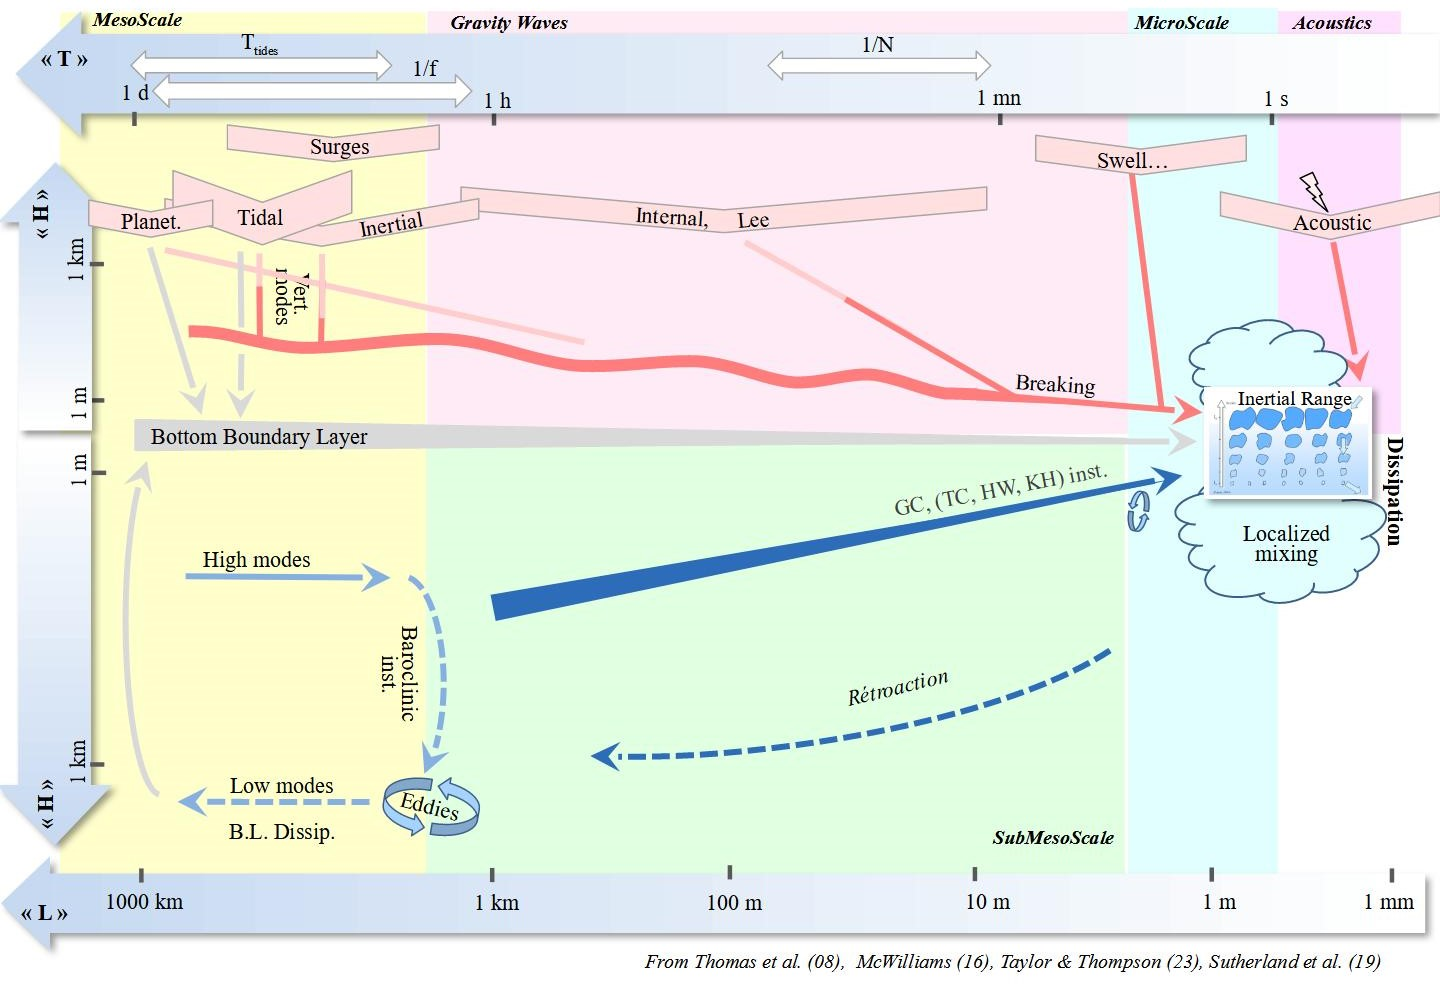
\includegraphics[width=1
    \textwidth]{images/SMC.jpg}
    \caption{Processus de sous-mésoéchelle et cascade d'énergie. \\
    En abscisse on retrouve l'échelle spatiale horizontale caractéristique des phénomènes, en ordonnée c'est l'échelle verticale. \FAadd{La moitié supérieure de la figure concerne les ondes, la moitié inférieure les instabilités et les processus dynamiques autres que les ondes.} La flèche labellisée "T" représente elle l'échelle temporelle caractéristique. Les couleurs représentent les régimes dynamiques auquel appartiennent les processus (qui seront détaillés plus tard). Les flèches (pleines et pointillées) illustrent les phénomènes de \textit{cascading} entre les différentes échelles.}
    \label{fig:echelles}
\end{figure}

La figure \ref{fig:echelles} \FAadd{présente} les différents processus faisant le liens entre mésoéchelle, sous-mésoéchelle et microéchelle, dans l'océan et à sa surface. Pendant ce stage, nous nous sommes plus spécifiquement intéressés à différents types de processus et d'instabilités de sous-mésoéchelle: instabilités convectives, instabilités de cisaillement, mais aussi propagation des ondes acoustiques dans l'océan.
\\


\subsection{Bases dynamiques des processus}
\label{Dynamiques globales}
L'ensemble de la dynamique des phénomènes étudiés s'appuie sur les équations de la mécanique des fluides et de la thermodynamique :
\begin{equation}
    \frac{\partial \rho}{\partial t} = - \nabla \cdot (\rho \mathbf{v})
    \label{eq:continuite}
\end{equation}
\begin{center}
    \textit{Equation de continuité}
\end{center}
\begin{equation}
    \partial_t \rho \mathbf{v} = - \nabla (\rho \mathbf{v} \times \mathbf{v}) - 2\Omega \times \rho \mathbf{v} - \nabla p + \nabla (\mu (\nabla\mathbf{v} + \nabla\mathbf{v}^T) + \mu_2(\nabla \mathbf{v}) \mathbf{I}) +\rho \mathbf{g}
    \label{eq: qtt de mouvement}
\end{equation}
\begin{center}
    \textit{\textcolor{blue}{Equations du mouvement}}
\end{center}


\begin{equation}
    \partial_t \rho \theta = -\nabla(\rho\theta\mathbf{v}) + \nabla(\kappa_{\theta}\nabla\theta)
    \label{eq:chaleur}
\end{equation}
\begin{center}
    \textit{Equation de la chaleur}
\end{center}

\begin{equation}
    \partial_t \rho S = -\nabla(\rho S\mathbf{v}) + \nabla(\kappa_S\nabla S)
    \label{eq:salinite}
\end{equation}
\begin{center}
    \textit{Equation de la salinité} 
\end{center}
\begin{equation}
    \rho = \rho_{eos}(\theta , S, p)
    \label{eq:etat}
\end{equation}
\begin{center}
    \textit{Equation d'état}
\end{center}

\textit{Les termes des différentes équations  sont décrits dans l'Annexe 1 (\ref{Table_notations}).}
\\
Les équations du mouvement, de la chaleur et de la salinité \FAadd{(cite les labels... pour référence)} sont données sous forme \textit{flux} afin de faciliter leur interprétation en termes de bilan, anticipant de plus leur formulation numérique. \\

\vspace{0.5 cm}
Afin de faciliter la résolution numérique de ce système, la dépendance de la densité en la pression totale peut être linéarisée (Auclair et al., 2024)... En effet, on fait un développement limité autour de la pression hydrostatique $p_h$ :

\begin{equation}
    \rho_{eos}(\theta, S, p_h +\delta p) = \rho_{eos}(\theta, S, p_0) + c_s^{-2}(p_h - p_0) + c_s^{-2}\delta p+\mathcal{O}(\delta p^2)
\end{equation}
A l'ordre 0 en anomalie de pression totale $(\delta p)$, il est encore possible de décomposer le profil de densité en une composante (statiquement) stable $(\rho_h)$ et une composante instable $(\rho_c)$. Il est à noter que cette décomposition n'est pas unique mais qu'elle est obtenue via un algorithme de montée/descente demandant un minimum de calculs (auclair et al., 2024):
\begin{equation}
     \rho_{eos}(\theta, S, p_h +\delta p) \approx  \rho_h + \rho_c + c_s^{-2}\delta p
     \label{eq:decomp densite}
\end{equation}

\vspace{0.5 cm}

Ce modèle \FAadd{(1)-(5)} est suffisamment général pour simuler explicitement une vaste gamme de processus dynamiques, il peut toutefois être simplifié en ciblant une gamme d'échelles caractéristiques et en adimentionnalisant chacune des équations. Ceci nous permettra de définir ce qu'on appelle des "régimes dynamiques", c'est-à-dire un cadre avec des échelles caractéristiques des différentes variables. Ce sont les nombres adimensionnels (Reynolds, Rossby, Froude...) qui nous donneront des indications pour savoir dans quel régime nous nous trouvons.\\
Les processus étudiés sont répartis dans deux régimes dynamiques: le régime des ondes acoustiques et le régime de la turbulence stratifié. On montre en annexe les échelles caractéristiques associées à chaque régime.


\section{Le modèle Croco}
Croco (Coastal and Regional Ocean COmmunity model) est un code communautaire d'océan régional, côtier ou encore littoral (hilt, 2020). Croco s'appuie sur une formulation en différences et volumes finis et inclut des modules dynamiques, sédimentaires ou encore biogéochimique. \\


\subsection{Objectifs et hypothèses}
Au LAERO (Laboratoire d'Aérologie, Observatoire Midi-Pyrénées) l'équipe qui co-développe Croco se concentre sur la représentation dynamique et numérique des processus océaniques de sous-mésoéchelle. Cette équipe est plus spécifiquement en charge du noyau numérique non-hydrostatique et compressible en étroite collaboration avec l'équipe AIRSEA d'INRIA pour les aspects "calcul hautes performances" (Auclair et al., 2024).\\
Si l'objectif de ces développements demeure la simulation numérique réaliste de l'océan régional, les processus de sous-mésoéchelle sont toutefois systématiquement étudiés de façon isolée afin d'évaluer et faire évoluer l'ensemble des algorithmes et des schémas numériques. Des cas-tests académiques sont ainsi proposés et étudiés en détail d'un point de vue dynamique bien sûr mais aussi numérique et informatique (HPC...). L'étude spécifique des instabilités de cisaillement de type Kelvin-Helmholtz, \FAadd{est par exemple mise à profit pour aborder la simulation} LES\footnote{LES: Large Eddy Simulation, lorsque les grandes structures turbulentes menant à la cascade turbulente directe sont explicitement simulées.} avec le code Croco (Penney et al, 2020).
 On isole ainsi un processus et on \FAadd{le} représente de la façon la plus fidèle \FAadd{et la plus précise} possible, en cherchant un compromis avec le coût de calcul et plus généralement avec le coût environnemental de la simulation.
\\
Plusieurs hypothèses fondamentales ont été faites pour les représentations dynamiques, on parle notamment de représentation compressible et non-hydrostatique, deux hypothèses essentielles pour modéliser les ondes acoustiques. De plus, pour prendre en compte les ondes de surfaces, on considère l'existence d'un "toit libre", à l'inverse d'une surface océanique \FAadd{dite à toit rigide}. Le choix de remettre en cause l'hypothèse de Boussinesq et de rendre le code compressible n'est pas dicté par la seule prise en compte des ondes acoustiques mais aussi par la nécessité de rendre le code \textit{non-hydrostatique} (Auclair et al., 2018). En effet, sous l'hypothèse de Boussinesq, le calcul de la pression totale en écoulement non-hydrostatique requiert la résolution d'un système de Poisson tridimensionnel \FAadd{(ref ? Tu peux utiliser Auclair et al., 2011 si tu l'as déjà.. mais il y a bcp, bcp d'autres)}. La principale difficulté est dans ce cas liée au traitement de la surface libre et le choix fait dans le code Croco consiste à réintroduire les ondes acoustiques afin de conserver un système mathématiquement \textit{hyperbolique} et numériquement \textit{local} dans un contexte d'implémentation massivement parallèle \FAadd{dans un code à deux pas de temps}.



\subsection{Fonctionnement}
D'un point de vue plus informatique et plus spécifiquement en termes de \textit{Calcul Haute Performance} (en anglais HPC), le code océanique Croco est développé depuis le milieu des années 2010 par les équipes d'INRIA, du CNRS-INSU, d'IFREMER, du SHOM, de l'IRD et de l'Université de Toulouse III Paul Sabatier dans le cadre du Groupement de Recherche (GdR) éponyme. Cette communauté s'est à l'origine appuyée sur le code ROMS choisi avant tout pour ses excellentes performances en termes de coût de calcul mais aussi en termes de gestion optimale de la mémoire (\cite{shchepetkin_regional_2005}).\\
Comme son parent ROMS, Croco repose sur certains principes de fonctionnements tel que le calcul parallèle s'appuyant sur la bibliothèque MPI: au lieu d'utiliser l'ensemble des processeurs à disposition pour faire les calculs sur une grille entière, le type de calcul parallèle choisi permet de diviser la grille initiale en sous domaines sur l'horizontale et d'attribuer chaque sous-domaine à un processeur qui échangera ensuite ses informations avec les processeurs voisins. \\
Ensuite, concernant cette fois \FAadd{la grille de calcul et} les coordonnées verticales, CROCO s'appuie sur une grille Arakawa-C et un système de coordonnées dites "s" qui suivent à la fois l'évolution de la bathymétrie et celle de la surface libre au cours du temps. \\
A l'image de sa version d'origine (hydrostatique), le noyau numérique compressible et non-hydrostatique de CROCO repose sur un traitement séparé mais couplé (\textit{time-splitting} en anglais) de la dynamique lente (géostrophie, courants d'Ekman...) et de la dynamique rapide, cette dernière concernant essentiellement la surface libre et la physique compressible et non-hydrostatique. Un schéma temporel prédicteur/correcteur original dit \textit{LFAM3 / Forward-Backward} est implémenté (Shchepetkin \& McWilliams2005 et auclair 2024).\\

%%%%%%%%%%%%%%%%%%%%%%%%%%%%


%------------- Commandes utiles ----------------

\section{Les instabilités convectives}

Les processus étudiés dans cette partie sont abordés dans le cadre du régime de turbulences stratifiées (\ref{turbu strat}).
\subsection{L'instabilité de Rayleigh-Taylor}
\label{RT}
\FAdel{A l'instar de l'instabilité de Rayleigh-Taylor, l'instabilité convective se déclenche à l'interface entre deux fluides de densités différentes, lorsque le fluide de densité forte est au-dessus du fluide de densité faible. La stratification est alors statiquement instable.}
\FAadd{Proposition... Lorsque la stratification de l'océan est \textit{statiquement instable} (la masse volumique diminue avec la profondeur), de petites perturbations de cette dernière peuvent déclencher d'importants mouvements verticaux (on parle d'\textit{instabilité convective}). Lorsque cette instabilité se produit à l'interface entre deux masses d'eau de densité différentes (la plus dense se situant au dessus), on parle d'\textit{instabilité de Rayleigh-Taylor}.}\\ 


\subsubsection{Analyse dynamique}


Au sein de la décomposition proposée en \eqref{eq:decomp densite}, la composante $\rho_c$ est responsable du déclenchement de la convection. 
En l'absence de cette décomposition $(\rho_c=0)$, la convection peut toutefois être déclenchée de façon indirecte via l'action du gradient horizontal de pression hydrostatique puis de la composante compressible de ce même gradient de pression, ce choix de représentation sera étudié un peu plus loin (voir \ref{sans rhoc}). Une question sous-jacente repose alors sur les conséquences dynamiques de ce choix numérique et l'on peut se demander si le mélange induit est in fine identique dans les deux cas.\\


\vspace{0.5 cm}
Le terme clé dans la compréhension du phénomène de convection est la flottabilité. \\
On définit :
\begin{itemize}
    \item $\rho_0$ la densité de référence de Boussinesq
    \item $\rho_h$ le profil stable en densité
\end{itemize}
Dans ces conditions, on définit la flottabilité $b$ ainsi :
\begin{equation}
    b = \dfrac{-g}{\rho_0}\rho_c
\end{equation}

On voit donc le lien ici entre le mouvement vertical du fluide et la façon avec laquelle on décompose la densité. En effet la présence de $\rho_c$ installe un régime de convection immédiat, car on aura $b \neq 0$.\\

\subsubsection{Représentation numérique}

Le choix de cette décomposition de la densité est \FAadd{en outre} lié à  des problématiques numériques, nous allons voir tout de suite les différences dans le processus de la convection selon la représentation que l'on choisit. \\
Dans les deux cas, on part du même état initial, on considère un fluide stratifié et stable dans lequel on plonge une goutte stratifiée avec deux densités différentes. 

La représentation numérique nous montre une coupe verticale du processus, on suit l'évolution dans le temps de la densité du fluide, représentée par \textbf{la barre de couleur} de valeur minimale 20 unités arbitraires, et de valeur maximale 23. \FAadd{Ce sont bien des kg/m3 par rapport à $\rho_0$}

\begin{figure}[H]
    \centering
    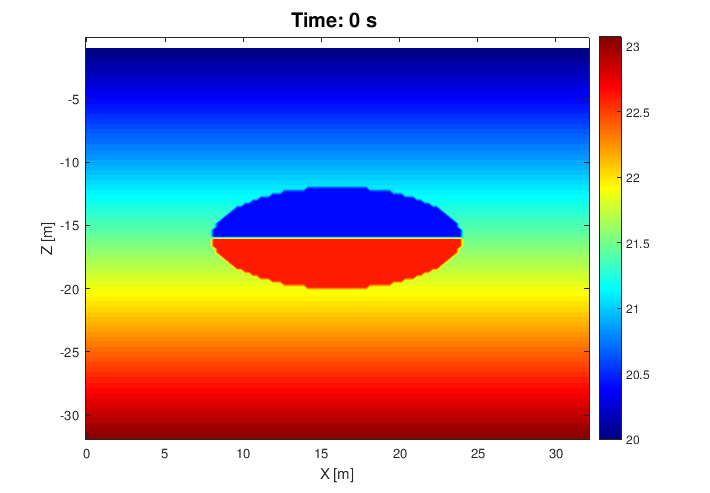
\includegraphics[width=0.7
    \textwidth]{images/Int_ConvT0.png}
    \caption{Instant initial}
\end{figure}


\vspace{1 cm}
\underline{\textbf{Avec le terme de convection :}}
\vspace{0.5 cm}

Dans ce cas de figure le terme $\rho_h$ est calculé afin de  lisser le profil de densité pour en faire un profil stable (voir section à préciser). Dans le code, il est calculé au pas de temps lent. \\
Ainsi, dans cette première configuration $\rho_c$ représente l'anomalie autour du profil stable, il est lui-aussi calculé au pas de temps lent. C'est donc ce terme qui déclenche la convection (cf équation (6)) via la flottabilité, terme de l'équation verticale du mouvement calculé cette fois au pas de temps rapide. \\

\begin{figure}[htb]
    \centering
    \subfloat[Etat du fluide au bout de 85 secondes]{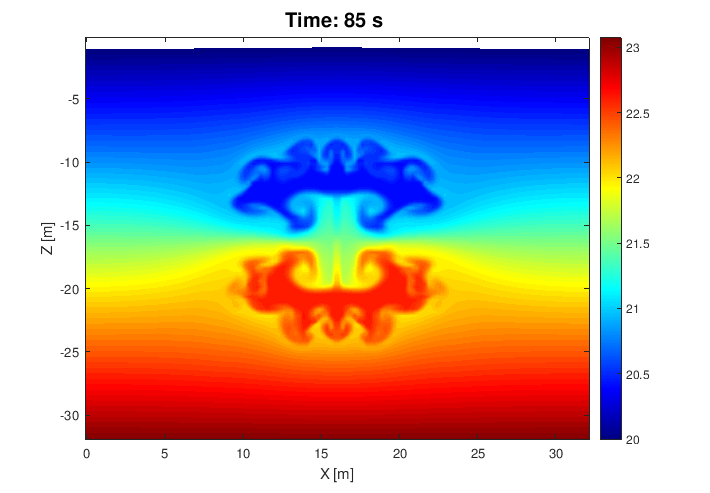
\includegraphics[width=0.45\textwidth]{images/avec_rhocS85.png}\label{fig:image1}}\hfill
    \subfloat[Etat du fluide au bout de 180 secondes. \\ Le mélange a débuté.]{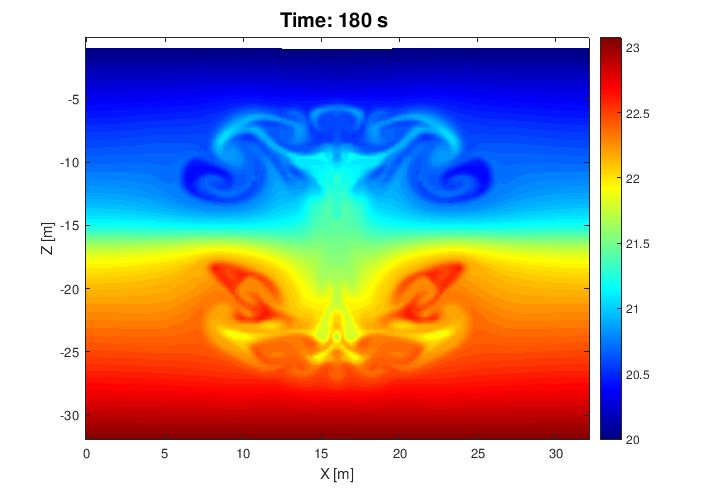
\includegraphics[width=0.45\textwidth]{images/avec_rhocS180.png}\label{fig:image2}}
    \caption{Représentation numérique de l'instabilité de Rayleigh-Taylor avec le terme $\rho_c$, où les couleurs représentent la masse volumique du fluide, pour des valeurs allant de 20 à 23 unités arbitraires.  \FAadd{kg/m3}}
    \label{fig:images_cote_a_cote}
\end{figure}

Au bout de 85 secondes, nous arrivons à distinguer une forme de champignon \FAadd{le long de l'interface entre la goutte et le fluide environnant}: c'est la forme caractéristique de l'instabilité de Rayleigh-Taylor. On remarque également des sortes de "vagues" autour du champignon (structures se développant cette fois \FAadd{le long de l'interface dans les régions présentant de forts gradients de vitesses}), ce sont des instabilités secondaires de Kelvin-Helmholtz, qui seront traitées plus tard (Cf \ref{KHI}).


\vspace{1 cm}


\underline{\textbf{Sans le terme de convection :}} 
\label{sans rhoc}
\vspace{0.5 cm}

Lorsque la décomposition de la densité ne fait pas apparaître le terme $\rho_c$, on a donc :
\begin{equation}
    \rho_{eos} = \rho_h + c_s^{-2}\delta p
\end{equation}
L'action conjointe des composantes hydrostatiques et non-hydrostatiques du gradient de pression est à l'origine de forts cisaillements de courant le long de la surface externe de la \FAadd{goutte}. En présence de stratification, des instabilités de cisaillement de type Kelvin-Helmholtz se déclenchent. Ces instabilités sont étudiées en détail par la suite (Cf \ref{KHI}).
\\
La simulation numérique donne :

\begin{figure}[H]
    \centering
    \subfloat[Etat du fluide au bout de 85 secondes]{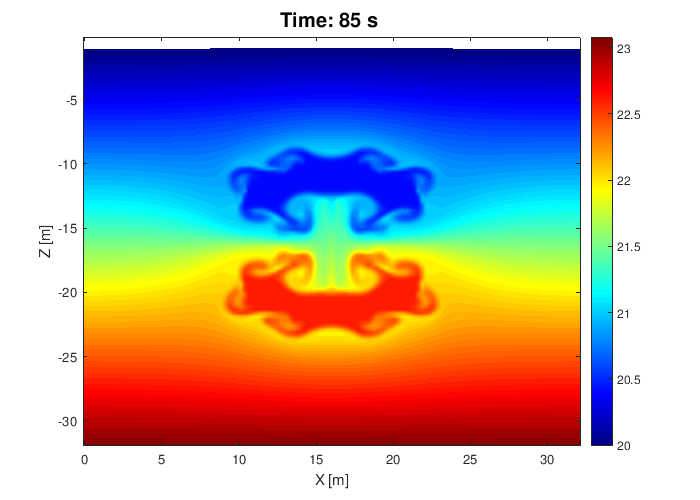
\includegraphics[width=0.45\textwidth]{images/sans_rhocS85.png}\label{fig:image1}}\hfill
    \subfloat[Etat du fluide au bout de 180 secondes. \\ Le mélange a débuté.]{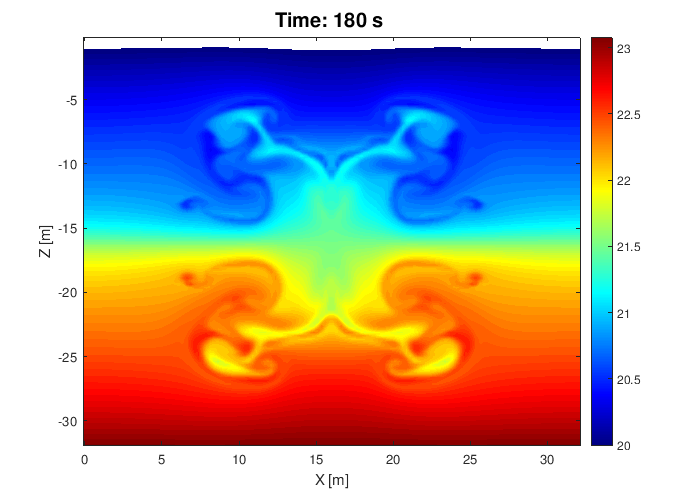
\includegraphics[width=0.45\textwidth]{images/sans_rhocS180.png}\label{fig:image2}}
    \caption{Représentation numérique de l'instabilité de Rayleigh-Taylor sans le terme $\rho_c$, où les couleurs représentent la masse volumique du fluide, pour des valeurs allant de 20 à 23 unités arbitraires (\FAadd{kg/m3}).}
    \label{fig:images_cote_a_cote}
\end{figure}
\underline{\textbf{Conclusion partielle :}} \\
\vspace{0.5 cm}

On remarque des différences dans le développement du processus, notamment dans l'étendue verticale de la convection. On retrouve quand même les instabilités secondaires de Kelvin-Helmholtz, qui viennent du cisaillement des vitesses. \FAadd{Ces instabilités ne sont pas toutefois pas localisées dans les mêmes régions et sont en nombre plus restreint avec le terme de convection.}    
On voit que le mouvement a une extension verticale beaucoup plus restreinte que lorsque la décomposition de $\rho$ prenait en compte $\rho_c$. \\
Nous ne l'avons pas montré ici mais, \FAadd{à plus long terme, en fonction de la représentation numérique} que l'on choisit, nous n'obtenons pas le même mélange final dans les deux cas. On comprent ainsi l'importance de bien représenter ce processus, même si on est seulement intéressé par l'état final, i.e. une fois le \textit{mélange diapycnal} terminé.
\\


\subsection{L'instabilité de Kelvin-Helmholtz}
\label{KHI}

Cette instabilité se produit au niveau d'une interface de cisaillement de vitesse dans un fluide stratifié (c'est-à-dire, $N = cste$). Elle fait partie de la famille des instabilités de cisaillement de la sous-mésoéchelle, avec les instabilité de Taylor-Caulfield et de Holmboe-Wave (\cite{shear_instabilities_2018}).
\\

\subsubsection{Analyse dynamique}

On considère un fluide stratifié dans lequel on retrouve un cisaillement de vitesse. Plus précisément, sur la figure \ref{fig:KHI1} \FAadd{la masse d'eau légère localisée dans la partie supérieure (en bleu)} a une composante horizontale de vitesse égale à $+1 m \cdot s^{-1}$, tandis que la masse d'eau légère (en rouge) vaut $-1 m \cdot s^{-1}$. D'un point de vue statique, \FAadd{les colonnes d'eau sont stables:} $\rho_{bleu} < \rho_{rouge}$. \\
On exprime la vitesse du fluide sous la forme d'une anomalie autour du profil moyen U, on a donc $u = U+u'$ avec $\|u'\|<<\|U\|$. \\
On se place également sous l'hypothèse incompressible, ce qui nous permet d'écrire: 
\begin{equation}
    \mathbf{\nabla} \cdot \mathbf{u} = 0
\end{equation}
Ainsi, nous pouvons réécrire les équations de la mécaniques des fluides et de la thermodynamique \FAadd{(section \S \ref{Dynamiques globales})} en fonction de $\psi$, la fonction de courant afin de réduire le nombre d'inconnues au prix d'une équation d'évolution présentant des dérivées partielles d'ordre plus élevé. \FAadd{$\Psi$ est définie par: (...) Cite de plus Valis (par exemple).}
\\
On écrit :
\begin{equation}
    \psi(x,y,t) = \tilde{\psi}(y)exp(ik(x-ct))
    \label{eq: fct courant}
\end{equation}
Nous obtenons donc l'équation de Taylor-Goldstein, après avoir remplacé $u$ par les différentielles de $\psi$ dans le système d'équation \ref{Dynamiques globales}: \\
\begin{equation}
    (U - c)( \partial_{zz}\tilde{\psi} - k²\tilde{\psi}) + (\frac{N²}{U - c} - \partial_{zz} U)\tilde{\psi} = 0
    \label{eq: taylor goldstein}
\end{equation}
\FAadd{Attention toutes les notations doivent ici être définies...}

Comme écrit au début du paragraphe, d'un point de vue statique, le fluide est stable, il faut dont que l'instabilité soit \textbf{déclenchée} \FAadd{Dit autrement... le moteur de cette instabilité est le cisaillement de vitesse.} \\

La stratégie adoptée pour mettre en évidence un critère de stabilité est la suivante : on rend $c$ complexe c'est à dire qu'on pose: $c = c_r + ic_i $. Ainsi, le système sera instable seulement si $c_i \neq 0$. Plus précisément, c'est le signe de $c_i$ qui nous indiquera la stabilité du système, le fait qu'il ne soit pas égal à 0 ne permet pas de le déterminer. \FAadd{Attention, il manque un élément dans ton raisonnement associé au théorème de Squire (équation à coef réel avec invariance par renversement du temps: si ($\psi, c$) est solution, alors ($\psi^*, c^*$) l'est aussi (*=conjugué). Ce qui veut dire que s'il y a une solution non triviale stable, il y a aussi une solution non triviale instable.}

Cependant, en retravaillant l'équation de Taylor-Goldstein \eqref{eq: taylor goldstein} et en supposant que $c_i \neq 0$, on obtient une condition nécessaire à remplir pour déclencher l'instabilité:
\begin{equation}
    N^{2} - \frac{1}{4}(\frac{\partial U}{\partial z})^{2}  < 0
\end{equation}
En fait, cette condition a 2 solutions, une stable (pas de d'instabilité de Kelvin-Helmholtz donc) et une instable (celle qui nous intéresse), c'est pour cela qu'on qualifie cette condition de nécessaire non suffisante.\\
Le critère nécessaire d'instabilité est donc: $\dfrac{N^2}{(\frac{\partial U}{\partial z})^2} < \dfrac{1}{4}$, que l'on peut traduire par :

\begin{equation}
    Ri < \frac{1}{4}
\end{equation}
\FAadd{Si tu manques de place dans ton rapport, tu peux déplacer cette démonstration en annexe... et citer un ouvrage tel que Vallis. Une petite "fiche" en annexe montrera quoiqu'il en soit ton investissement et fait que tu es allée au bout du raisonnement.}

\subsubsection{Représentation numérique}
Le processus de mélange par instabilité de Kelvin-Helmholtz se déroule en plusieurs étapes. Tout d'abord après quelques secondes à peine on distingue la phase \textbf{d'enroulement} (voir figure \ref{fig:KHI2}), la partie la plus dense du fluide s'enroule autour de la partie moins dense ce qui forme une sorte de vague. Ensuite, le \FAadd{ce filament} s'étire donc, par conservation de matière puis \FAadd{le filament} s'amincit, c'est la phase \textbf{d'étirement} (figure \ref{fig:KHI3}). A ce stade, aucun processus diabatique n'est véritablement entré en jeu), il n'y a pas de mélange, on voit encore bien les phases bleues et rouges du fluide, ce n'est qu'après la phase d'étirement que le mélange se fait (figure \ref{fig:KHI4}) \FAadd{et que les processus proprement diabatiques entrent en jeu}.
\begin{figure}[htbp] % L'argument [htbp] indique à LaTeX d'essayer de placer la figure "ici", "en haut de la page", "en bas de la page" ou "à la page suivante", selon ce qui convient le mieux.
    \centering
    \begin{minipage}{0.45\textwidth}
        \centering
        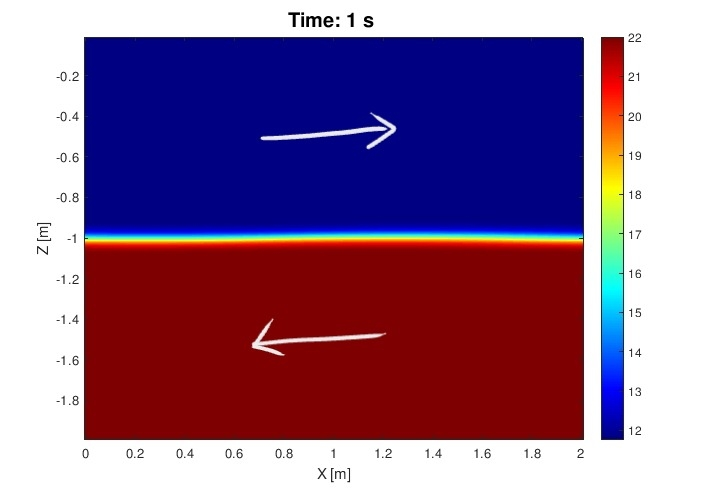
\includegraphics[width=\linewidth]{images/KHI1.png}
        \caption{Etat initial}
        \label{fig:KHI1}
    \end{minipage}
    \hspace{0.05\textwidth} % Espace horizontal entre les deux images
    \begin{minipage}{0.45\textwidth}
        \centering
        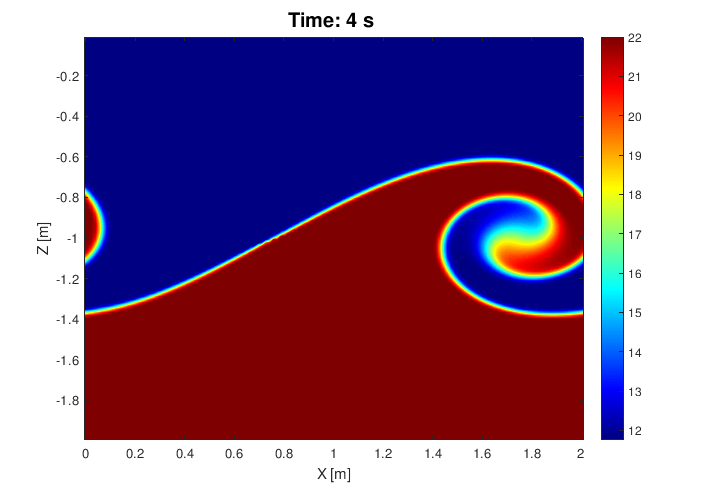
\includegraphics[width=\linewidth]{images/KHI2.png}
        \caption{Phase d'enroulement}
        \label{fig:KHI2}
    \end{minipage}
    \begin{minipage}{0.45\textwidth}
        \centering
        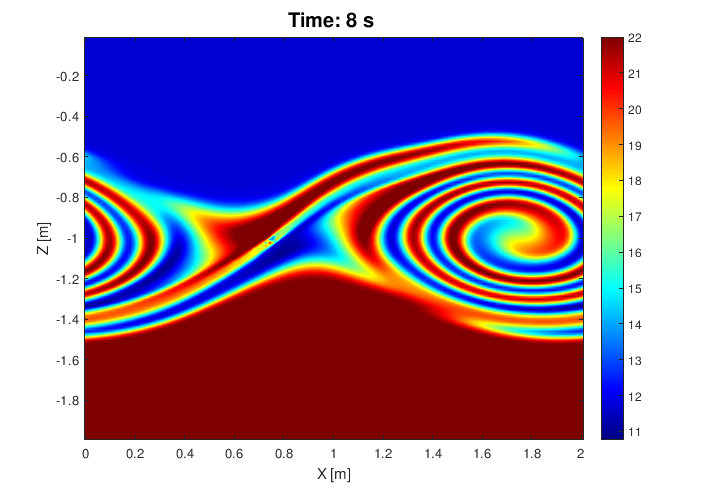
\includegraphics[width=\linewidth]{images/KHI3.png}
        \caption{Phase de brassage}
        \label{fig:KHI3}
    \end{minipage}
    \hspace{0.05\textwidth} % Espace horizontal entre les deux images
    \begin{minipage}{0.45\textwidth}
        \centering
        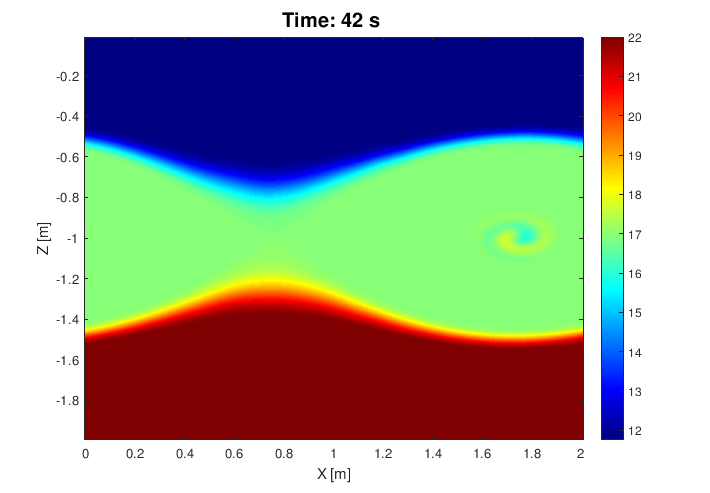
\includegraphics[width=\linewidth]{images/KHI4.png}
        \caption{Mélange}
        \label{fig:KHI4}
    \end{minipage}
    \caption{Etapes d'évolution de l'instabilité de Kelvin-Helmholtz, où les couleurs représentent la masse volumique du fluide, pour des valeurs allant de 11 à 22 unités arbitraires.}
\end{figure}
\\
\vspace{0.5 cm}

\underline{\textbf{Conclusion partielle :}} \\
\\


Finalement on a réussi à bien représenter le processus et ses différentes phases. \FAdel{En effet on note une bonne correspondance entre la théorie et la simulation, la longueur d'onde utilisée dans le modèle correspond bien à la valeur attendue, on le voit grâce aux dimensions horizontales qui capturent parfaitement une motif du phénomène (évitant ainsi des coûts environnementaux non nécessaires ici).}
\FAadd{On montre en particulier (Penney et al., 2021 et M. Andrieux, manuscrit de thèse en cours de rédaction, communication personnelle), que la longueur d'onde $(2\pi/k)$ la plus instable (pour laquelle la croissance de l'instabilité est la plus forte) correspond à celle prédite par l'analyse de l'équation de Taylor-Goldstein.}
\\

\section{Les ondes acoustiques: propagation en océan stratifié}

Nous allons maintenant nous intéresser à la propagation des ondes acoustiques dans l'océan. \FAadd{Nous avons vu que les ondes acoustiques avaient été réintroduites dans le code Croco afin de simuler explicitement les processus non-hydrostatiques. Croco ayant été rendu compressible par choix numérique et algorithmique, ce code propage donc les ondes acoustiques et peut ainsi être utilisé en acoustique sous-marine dans un contexte océanique réaliste. Notons que dans sa version actuelle, le code Croco permet d'étendre la grille de calcul au sédiment se trouvant sous le fond océanique afin de propager les ondes acoustiques dans les couches sédimentaires.
Des applications intéressantes en découlent } notamment dans la prévention des risques lors de la génération d'évènements potentiellement catastrophiques tels que les tsunamis. Effectivement, les ondes acoustiques générées lors de la mise en mouvement initiale de la colonne d'eau par les forçages du tsunami, se déplacent dans l'océan à une vitesse d'environ 1 500 $m \cdot s^{-1}$, à titre de comparaison \FAadd{l'onde de surface} d'un tsunami peut se déplacer à 200 $m \cdot s^{-1}$ \FAadd{(pour un océan de 4000 m de profondeur)}. Ainsi, trouver une caractérisation acoustique de ces phénomènes pourrait améliorer leur détection et donc dans ce cas précis anticiper l'évacuation de la population.

\subsection{Postulats dynamiques}
\subsubsection{Mise en équation}


On repart du système d'équations présenté en introduction (voir \§ \ref{Dynamiques globales}). Nous nous plaçons ici dans le cadre des approximations et des échelles données par le régime des ondes acoustiques (\ref{ondes acous}). D'ailleurs, nous remarquons que la période temporelle caractéristique du phénomène est bien plus grande que celle des instabilités étudiées plus tôt.
\\
Dans l'étude de ce processus, on néglige la force de Coriolis, la viscosité et le coefficient de diffusivité. Par contre on conserve par la seconde viscosité (moléculaire) liée à la dissipation de l'onde acoustique et ce en particulier dans le sédiment.
\\
Ce n'est pas une équation de d'Alembert classique que vérifie la pression ici, en effet il faut prendre en compte la vitesse et la non-homogénéité du fluide. Voici l'équation que propose Oleg Godin pour la propagation d'une onde acoustique dans un milieu non borné: (\cite{godin_wave_2011}) 
\begin{equation}
    \frac{d}{dt}[\frac{d}{dt}(\frac{1}{\rho c²}\frac{dp}{dt}) - \nabla \cdot \frac{\nabla p}{\rho}] + 2\frac{\partial \mathbf{u}}{\partial x_i} \cdot \nabla (\frac{1}{\rho}\frac{\partial \rho}{\partial x_i}) = 0
\end{equation}

Cependant, cette équation ne retranscrit qu'une partie de ce qu'on cherche à représenter. En effet, nous souhaiterions prendre en compte les conditions aux limites: les sédiments au fond de l'océan et à la surface libre, car celles-ci sont essentielles pour comprendre le concept de propagation en modes. 

\subsubsection{Concept de modes de propagation}

A la manière de la propagation d'une onde électromagnétique dans une fibre optique, l'onde acoustique ici se réfléchit à la fois à la surface et au fond de l'océan. Cela conduit notamment à des interférences entre les différents fronts réfléchis. Les interférences constructrices forment ce qu'on appelle des "modes de propagation". On numérote également ces modes: les numéros correspondent au nombre de réflexion avant l'interférence. On comprend donc que plus le mode est élevé, moins le front est rapide.\\
En plus de la réflexion de l'onde, les conditions aux limites ont des conséquences particulières sur la propagation de celles-ci. En effet dans le cas de l'océan l'onde se propage plus vite dans le sédiment, donc \FAadd{dans le couche} inférieure (\cite{CL_acous_2015}). \FAdel{On peut donc voir des "bribes d'ondes", venues de la réfraction entre sédiment et océan être en avance sur les premiers modes de propagation.}


\\
D'ailleurs, on montre que les propagations en modes respectent les relations de dispersions qu'on obtient analytiquement (thèse de Pierre-Antoine Dumont en cours de rédaction, communication personnelle).

\subsection{Propagation en 2d dans un océan stratifié en prenant en compte la bathymétrie}


\subsubsection{Cas général avec une bathymétrie marquée}

\begin{figure}[H] % L'argument [htbp] indique à LaTeX d'essayer de placer la figure "ici", "en haut de la page", "en bas de la page" ou "à la page suivante", selon ce qui convient le mieux.
    \centering
    \begin{minipage}{0.45\textwidth}
        \centering
        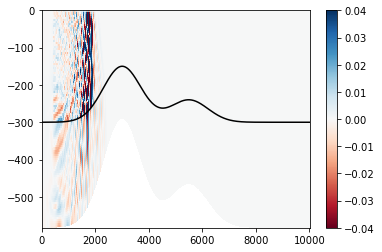
\includegraphics[width=\linewidth]{images/im2.png}
        \caption{Image 1}
        \label{fig:image1}
    \end{minipage}
    \hspace{0.05\textwidth} % Espace horizontal entre les deux images
    \begin{minipage}{0.45\textwidth}
        \centering
        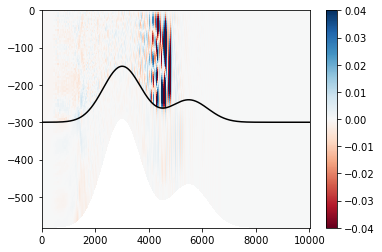
\includegraphics[width=\linewidth]{images/im4.png}
        \caption{Image 2}
        \label{fig:image2}
    \end{minipage}
    \vspace{1cm} % Espace vertical entre la première ligne et la deuxième image
    \begin{minipage}{0.9\textwidth}
        \centering
        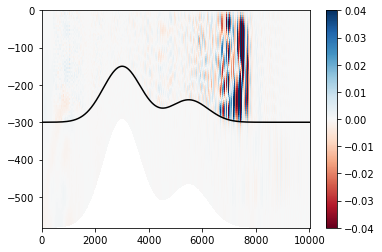
\includegraphics[width=0.45\textwidth]{images/im6.png}
        \caption{Image 3}
        \label{fig:image3}
    \end{minipage}
    \caption{Propagation de l'onde acoustique. En ordonnée la profondeur en mètres, avec la ligne de bathymétrie, en abscisse la dimension spatiale horizontale.}
    \label{fig:three_images}
\end{figure}
Pour la première configuration, on considère une onde acoustique émise à 100 m de profondeur, dans un environnement avec une bathymétrie \FAadd{non constante}. \\
\FAadd{Les modes sont visibles sur les figures.} \\
D'ailleurs, à  partir de la deuxième image on voit bien que l'onde se propage plus vite dans le sédiment que dans l'océan, on aperçoit également la réfraction de l'onde dans le sédiment qui retourne dans l'océan, qui se trouve donc devant le front d'onde.\\
\FAadd{On remarque également la plus forte atténuation de l'onde dans le sédiment.}

\\
\vspace{1 cm}

\FAadd{Dans un second temps, j'ai réalisé} des simulations en changeant à la fois la nature du sédiment (argile ou sable) mais aussi la profondeur de l'océan (150 et 300 mètres)
\subsubsection{Influence du sédiment}
On  compare la propagation d'une onde acoustique dans un océan de 150 m de profondeur en fonction de la nature du sédiment. \\
Pour l'argile (respectivement, pour le sable), on a pris une vitesse de compression de $1550 m \cdot s^{-1}$ (respectivement $1800 m \cdot s^{-1}$)  et une densité égale à $1.7 kg \cdot dm^{-3}$ (respectivement $2 kg \cdot dm^{-3}$).
\\
D'ailleurs la vitesse de compression dans un sédiment dépend entre autre de sa densité, plus le milieu est dense, plus l'onde se propage rapidement.
\begin{figure}[H]
    \centering
    \subfloat[Propagation dans un milieu argileux]{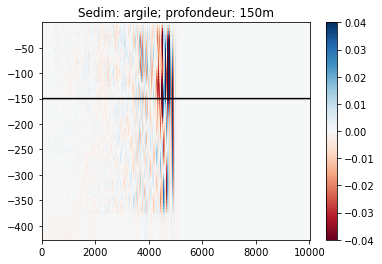
\includegraphics[width=0.45\textwidth]{images/im4_150_argile.png}}\label{fig:image1}\hfill
    \subfloat[Propagation dans un milieu sableux]{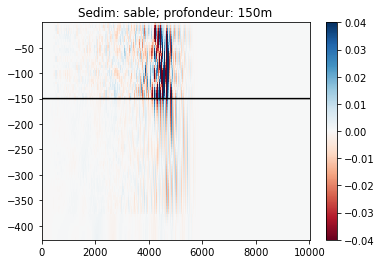
\includegraphics[width=0.45\textwidth]{images/im4_150_sable.png}\label{fig:image2}}
    \caption{Influence du sédiment dans la propagation d'une onde acoustique}
    \label{fig:images_cote_a_cote}
\end{figure}
Ainsi, comme on pouvait s'y attendre, l'onde se déplace plus vite dans le sable que dans l'argile. Cependant, il semblerait que le sable soit un milieu plus dispersif que l'argile dans la mesure où l'onde à l'air de s'atténuer beaucoup plus rapidement dans le milieu sableux.

\subsubsection{Influence de la profondeur}

\FAadd{J'ai enfin comparé} la propagation de l'onde dans un même milieu (ici avec un fond marin argileux) mais pour des profondeurs différentes. 

\begin{figure}[H]
    \centering
    \subfloat[Propagation dans un océan de 150 mètres de profondeur]{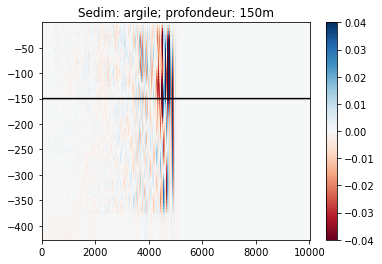
\includegraphics[width=0.45\textwidth]{images/im4_150_argile.png}}\label{fig:image1}\hfill
    \subfloat[Propagation dans un océan de 300 mètres de profondeur]{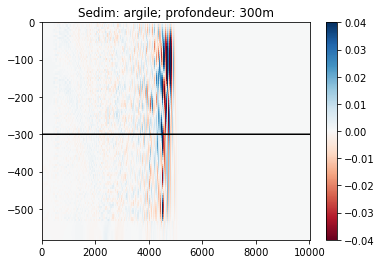
\includegraphics[width=0.45\textwidth]{images/im4_300_argile.png}\label{fig:image2}}
    \caption{Influence de la profondeur dans la propagation d'une onde acoustique}
    \label{fig:images_cote_a_cote}
\end{figure}
Dans l'océan profond de 150 m, l'onde semble complètement atténuée dans la couche sédimentaire vers une profondeur de -370 m. Pour celui profond de 300 m, l'onde résiste au delà de 500 m de profondeur. Globalement dans les deux océans les ondes sont atténuées dans le sédiment après une distance caractéristique approchant 200 m. \\
\\
\underline{\textbf{Conclusion partielle :}} \\
\\
Finalement, on comprend que plusieurs facteurs rentrent en jeu lorsqu'il s'agit d'évaluer la propagation d'une onde acoustique dans l'océan.
\FAadd{P.A. Dumont (manuscrit de thèse, communication personnelle a montré que la vitesse de propagation des modes acoustiques simulées avec Croco correspondait précisément à celle prédite théoriquement pour un guide d'ondes constitué d'une couche océanique et d'une ou plusieurs couches sédimentaires.}
D'autre part, la nature du sédiment influence la vitesse de propagation de l'onde, en effet l'onde se propage plus vite dans le sable, c'est-à-dire dans le milieu le plus dense (la masse volumique du sédiment n'est pas le seul paramètre à prendre en compte).\\
\FAdel{D'un point de vue cette fois plus global, des processus modifiant les paramètres physiques de l'océan (comme les instabilités que nous avons étudiées) surviennent constamment, il est donc nécessaire de savoir comme ces perturbations se propagent dans ce milieu, pour appréhender au mieux les nouvelles conditions initiales pour un nouveau processus.}
\FAadd{Rappelons enfin que la qualité et la précision de la propagation des ondes acoustiques dans Croco ne sont pas seulement des problèmatiques d'acoustique sous-marine. Ces ondes jouent évidemment un rôle essentiel dans l'ajustement des processus océanique basse-fréquences.} La propagation des perturbations de pression totale se fait entre autre par les ondes acoustiques, d'où l'importance de bien les représenter numériquement. \FAadd{L'étude de ces processus ondulatoires entre donc une nouvelle fois dans le cadre de l'étude et de la simulation explicite de la sous-mésoéchelle océanique}.\\
\FAadd{J'ai enfin participé à l'élaboration de fiches de synthèse sur les différents processus de sous-mésoéchelle, fiches utilisées par l'équipe pour documenter les recherches en cours et pour sa communication interne et externe.}\\


\section{Discussion et conclusion}

\FAadd{L'objectif de mon stage au LAERO était de m'immerger dans les recherches en cours sur la sous-mésoéchelle océanique. Après discussion avec les membres de l'équipe, j'ai sélectionné un certain nombre de processus fondamentaux pour lesquels j'ai simultanément et systématiquement cherché à travailler sur plusieurs aspects: la dynamique propre des processus bien sûr mais aussi les problèmes liés à leur simulation numérique explicite et au coût environnemental de leur représentation numérique. 
J'ai ainsi pu} étudier quelques processus clés de sous-mésoéchelle de natures différentes \FAdel{des instabilités convectives qui changent les caractéristiques physiques d'un milieu et la propagation de ondes acoustiques, donc de ces variations.}  \FAadd{ et j'ai plus spécifiquement choisi de concentrer mon étude sur deux types d'instabilités (l'instabilité convective et l'instabilité de cisaillement) ainsi que sur la propagation des ondes acoustiques. 
J'ai ainsi compris que la dualité entre l'étude dynamique et la représentation numérique permettait d'évaluer la pertinence du modèle, de faire progresser notre connaissance des processus dynamiques}, mais aussi de mettre en évidence certains biais à prendre en compte dans la modélisation de ces phénomènes, des biais qu'on aurait pas imaginés intuitivement (comme celui soulevé par la décomposition de la densité en \ref{RT} \FAadd{ou encore la présence de dissipation implicite associée à la représentation numérique de l'advection.) Une bonne connaissance des limites du protocole de modélisation est en fine tout aussi importante que ses qualités numériques intrinsèques.}


Cependant il manque encore quelques étapes pour passer de la modélisation isolée des processus océaniques à la représentation numérique d'un bassin. Effectivement la non-linéarité de l'océan implique que ce qu'il s'y passe ne peut pas se réduire à la simple somme des processus océaniques individuels. Ainsi, pour évaluer la pertinence du modèle \FAadd{une bonne connaissance de l'océan réel est indispensable, connaissance qui ne peut être fournie que par des observations} in situ par le biais des différentes campagnes de mesures par exemple. Ces campagnes étant coûteuses, à la fois financièrement et environnementalement, des observations en laboratoire sont également menées à bien, sur la plateforme Coriolis à Grenoble par exemple où on essaie de reproduire les conditions physiques de l'océan (rotation de la Terre, bathymétrie...).
\\
Finalement cette première expérience dans le monde de la recherche m'a permis de mieux appréhender le métier de chercheur et aussi de me conforter dans mes différents choix d'orientation. En effet mon stage s'étant situé à la frontière entre travail de recherche et travail de vulgarisation j'ai pu au moins apercevoir les qualités et les méthodes requises pour chercher et enseigner. En discutant avec les chercheurs, les doctorants et les ingénieurs de recherche j'ai aussi découvert comment la communauté interagissait pour étendre notre connaissance sur des sujets divers et variés, parfois au carrefour de plusieurs disciplines différentes. Ensuite, j'ai également pu explorer un peu plus en profondeur l'océanographie, en faisant écho au cours d'introduction du premier semestre. J'ai énormément aimé travailler dans ce domaine, cela m'encourage même à y effectuer mon stage de Master 1.


\newpage



% Ajout de l'annexe
\newpage
\begin{appendices}
\section{Annexe : }
Dans cette section de l'annexe, nous fournissons des détails supplémentaires.
\subsection{Définition des variables}
%%%%%%%%%%%%%%%%%%%%%%%%%%%%%
%%% Tableau des variables %%%
%%%%%%%%%%%%%%%%%%%%%%%%%%%%%
{\renewcommand{\arraystretch}{1.5}
\begin{table}
\begin{center}
\begin{tabular}{ l l }
\hline 
$\mathbf{g} = (0,0,g)$ &  accélération de la pesanteur \\
$\boldsymbol{\Omega} = (0,f^\perp/2,f/2)$ & vecteur de vitesse angulaire dans le référentiel local \\
%$\boldsymbol{\tau}$  & viscous stress tensor \\ 
$\nabla = (\partial_x, \partial_y, \partial_z)$ & opérateur gradient en coordonnées cartésiennes\\
$\mathbf{\nabla}_{\mathscr{s}}.(\rho h \mathbf{v})= \partial_{x} \rho h u \big\vert_\mathscr{s}+\partial_\mathscr{s}\rho v_\mathscr{s}$ & Advection exprimée en terme de flux  \\
\hline
$\mathbf{v} = (u,v,w)$, $\mathbf{u} = (u,v,0)$  & vecteur vitesse en 3D , vecteur vitesse horizontale  \\ 
$(\theta,\rho,S)$ & Température potentielle, densité et salinité \\
$L_h$ & échelle spatiale horizontale \\
$\psi$ & fonction de courant \\
$\rho_0$  &  densité de référence de Boussinesq \\
$p_0(z) = - \rho_0 g z$ & pression de référence   \\
$p_{\rm h}=-\rho_{\rm h} g$  & pression hydrostatique\\
$\rho_{\rm c} = \rho_{\rm eos}(\theta,S,p_0)-\rho_h$  & partie instable de la densité \\
$\delta p=c_s^2\delta\rho$  & pression compressible et anomalies de densité avec $c_s$ la vitesse de propagation du son \\
$N = \sqrt{-\dfrac{g}{\rho_{\theta}}\dfrac{d\rho_{\theta}}{dz}}$ & fréquence de Brunt-Vaisala avec $\rho_{\theta}$ la densité potentielle \\
\hline
$\mu$ ($\mu_2$)  & viscosité dynamique \\
$\kappa_\theta$ ($\kappa_S$) & diffusivité thermique (du sel)\\
\hline 
\end{tabular}
\end{center}
\caption{\textit{définition des variables}}
\label{Table_notations}
\end{table}
}
%%%%%%%%%%%%%%%%%%%%%%%%%%%%%
%%% Tableau des variables %%%
%%%%%%%%%%%%%%%%%%%%%%%%%%%%%

\newpage 

\subsection{Nombres adimensionnels}
Afin de simplifier le système d'équation \ref{Dynamiques globales} en fonction des cas, nous faisons apparaître des nombres caractéristiques en rendant les équations adimensionnelles. Voici les nombres qui nous intéressent :
\begin{itemize}
    \item le nombre de Rossby: $Ro = \dfrac{U}{fL_h}$
    \item le nombre de Richardson: $Ri = \dfrac{N^2}{(\frac{\partial U}{\partial z})^2}$
    \item 
\end{itemize}

\subsection{Régimes dynamiques}
\subsubsection{Turbulences stratifiées}
\label{turbu strat}
Dans ce régime dynamique, on a : 
\begin{itemize}
    \item $Ro \approx 1$
    \item $T \approx \dfrac{L_h}{U}$
    \item $\rho \approx \rho_h + \rho_c$
    \item $\dfrac{\partial v_h}{\partial t} \approx \dfrac{-1}{\rho_h}\nabla p$
\end{itemize}

\subsubsection{Ondes acoustiques}
\label{ondes acous}
Dans ce régime, on a :
\begin{itemize}
    \item $Ro > 1$
    \item $T \approx \dfrac{L_h}{c_s}$
    \item $p \approx \delta p$
    \item $P \approx c_s^2 \delta \rho$
    \item $\partial_t \rho_c \approx \dfrac{N^2}{g}\rho_h w$
\end{itemize}


\end{appendices}

\end{document}